\section{Conexión con distintas teorías.}\label{seccion7}
\begin{center}
	\item \subsection{Teoría de grafos:}
\end{center}

\underline{\textbf{Definición:}}\\
Un \textbf{grafo} es un par $ (V,A) $ de conjuntos, junto con la aplicación 
\begin{center}
	 $  \gamma :A \rightarrow$ \{\{$u,v$\} / $u,v \in V$\}  
\end{center}
Al conjunto de puntos V se se llama conjunto de vértices y al conjunto A le llamaremos conjunto de aristas. \\

\underline{\textbf{Definición:}}\\
Un \textbf{grafo plano} $ G $ es un grafo que permanece en el plano.\\

Podemos ver varios ejemplos en la figura \ref{graf1}.\\
\begin{figure}[h!]
	\centering
	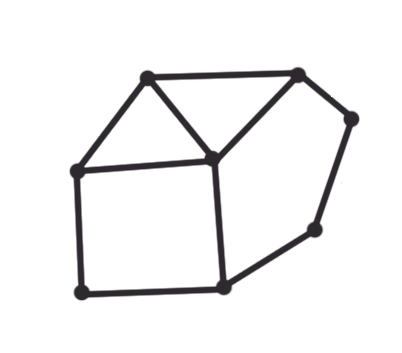
\includegraphics[width=3.5cm]{inudos/grafo.png}
	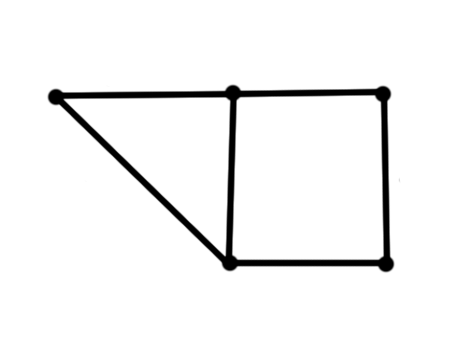
\includegraphics[width=4cm]{inudos/pgrafo.png}
	\caption{Ejemplos de grafos planos.}
	\label{graf1} 
\end{figure}

A partir de la proyección de un nudo (o de un enlace en general) podemos generar su grafo plano asociado. Para ello tendremos que realizar el siguiente proceso:\\

Sombreamos las regiones de la proyección que estén de modo que la región externa al nudo se quede sin sombrear y situamos un vértice en cada zona. Unimos los vértices con aristas que pasan por los cruces de la proyección. Ya tendríamos el grafo plano. Además, si el nudo tiene asignada una orientación, podremos asignarle el tipo de cruce (positivo o negativo) a cada arista. Podemos ver un ejemplo en la figura \ref{graf2}.\\
\begin{figure}[h!]
	\centering
	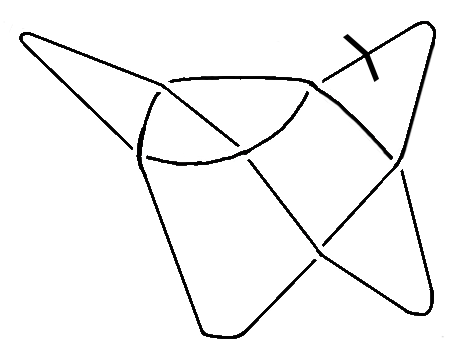
\includegraphics[width=5cm]{inudos/pgrafo3.png}
	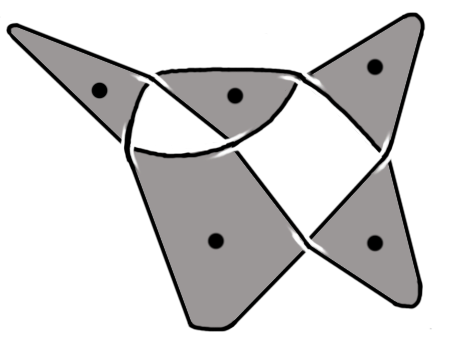
\includegraphics[width=5cm]{inudos/pgrafo2.png}
	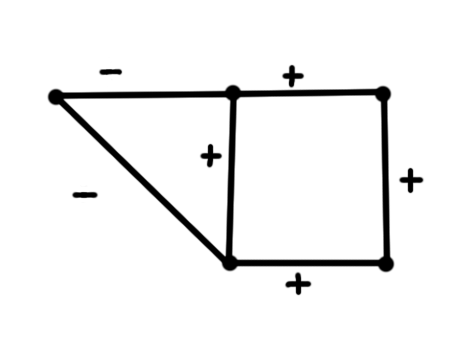
\includegraphics[width=5cm]{inudos/pgrafo1.png}
	\caption{De proyección a grafo}
	\label{graf2} 
\end{figure}

Finalmente, para ver que los problemas de nudos se pueden ver como problemas de grafos y viceversa, vamos a ver el procedimiento inverso. Dado un grafo plano, podremos obtener la proyección del nudo asociado. Veamos cuál sería el procedimiento:\\

Partiendo del grafo plano con los signos asociados en cada vértice, marcamos cada una de las aristas. Uniremos cada una de estas marcas con aquellas marcas que estén en las aristas que conectan con los vértices de la arista que tiene la marca. A continuación, sombreamos las zonas que contienen a cada vértice. Finalmente, establecemos los cruces conforme a los signos del grafo plano. Podemos ver un ejemplo en la figura \ref{graf3}.\\
\begin{figure}[h!]
	\centering
	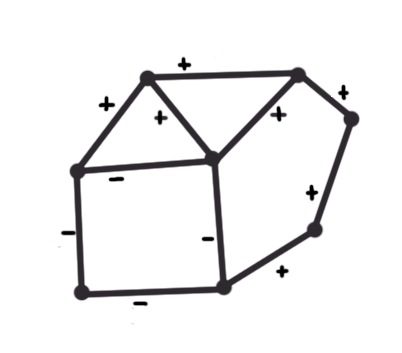
\includegraphics[width=4.5cm]{inudos/grafo1.png}
	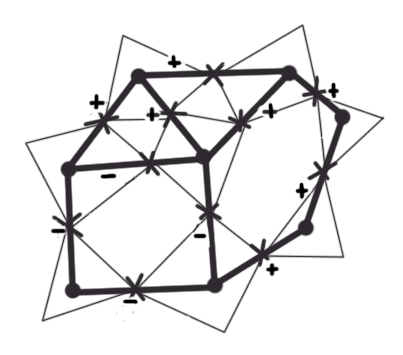
\includegraphics[width=4.5cm]{inudos/grafo2.png}
	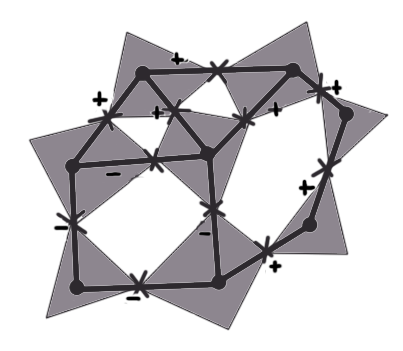
\includegraphics[width=4.5cm]{inudos/grafo3.png}
	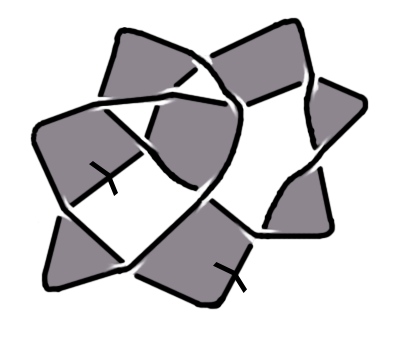
\includegraphics[width=4.5cm]{inudos/grafo4.png}
	\caption{De grafo a proyección.}
	\label{graf3} 
\end{figure}



\begin{center}
	\item \subsection{Teoría de trenzas:}
\end{center}
En esta sección vamos a introducir la relación que hay entre teoría de nudos y teoría de trenzas, teoría que estudiaremos con mayor detalle en el próximo tema.\\

Vamos a ver la idea general de lo que se entiende por el término trenza y veremos una definición más precisa más adelante. Podemos pensar en una trenza como un conjunto de $n$ cadenas que son atadas a un tope imaginario arriba y abajo. Podemos ver algunos ejemplos de trenzas en la figura \ref{ntren1}.\\
   \begin{figure}[h!]
   	\centering
   	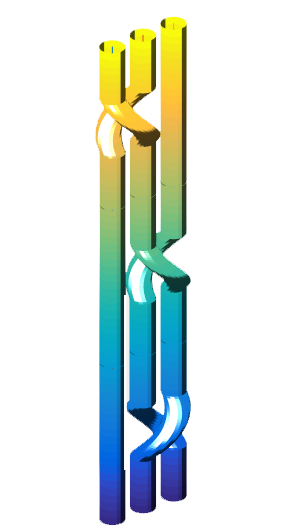
\includegraphics[width=3.5cm]{itrenzas/t4.png}
   	\space
   	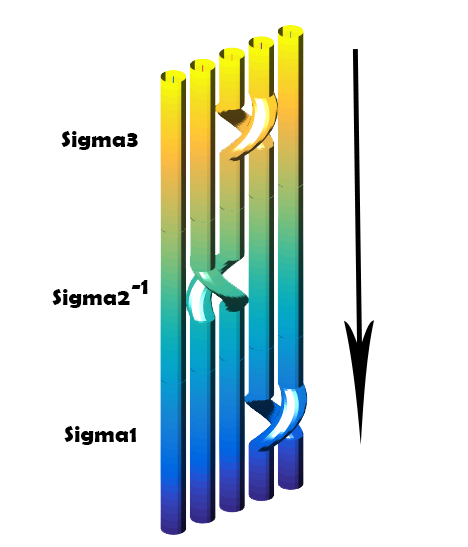
\includegraphics[width=6cm]{itrenzas/t7.png}
   	\caption{Ejemplos de trenzas}
   	\label{ntren1} 
   \end{figure} 

A partir de una trenza, podemos obtener su nudo o enlace correspondiente. Simplemente tendremos que unir en orden  los topes superiores de las cadenas con los inferiores. Esta trenza cerrada será el nudo al que representa la trenza. Podemos ver algunos ejemplos en la sección \ref{t2sec1}.\\

Para ver el proceso inverso haremos uso del siguiente teorema:
\begin{teo}Teorema de Alexander.\\
	Todo nudo puede ser representado como una trenza cerrada.
\end{teo}
//PENDIENTE DEMOSTRACIÓN A PARTIR DE POSIBLE IMPLEMENTACIÓN!!!!!!!!!!!!!!!!!!!!!

